% --
% adversarial training

\section{Experiments on Adversarial Pre-Training}\label{sec:exp_adv}
\thesisStateNotReady
Adversarial pre-training as already described in detail in \rsec{nn_adv} is the transfer of learned weights obtained from adversarial training between a Generator (G) and a Discriminator (D) network.
The target neural network architecture used for adversarial pre-training is the \texttt{conv-jim} model, described in \rsec{nn_arch_cnn}, obtaining pre-trained weights from its GAN versions the \texttt{adv-d-jim} and \texttt{adv-g-jim}, described in \rsec{nn_arch_adv}.
Note that frame-based normalization was applied, which made the training of GANs considerably more easy and the weights from the Generator network applicable.
Both adversarial pre-training techniques, the adversarial label and dual train explained in \rsec{nn_adv} were evaluated.

Note that the experiments in this section, like in the previous section, are not meant for comparison to the benchmark networks, because of a usage of 500 examples per label instead of the whole dataset.


% --
% label train

\subsection{Impact of Adversarial Label Train}\label{sec:exp_adv_label}
The adv-label-train experiments on the \texttt{conv-jim} architecture with obtained weights from either \texttt{adv-g-jim} or \texttt{adv-d-jim} are shown in \rtab{exp_adv_label_l12}.
\begin{table}[ht!]
\small
\begin{center}
\caption{Experiment with adversarial label pre-training, using either Generator \enquote{g} or Discriminator \enquote{d} weights.}
\begin{tabular}{ M{2cm}  M{2cm}  M{2.5cm}  M{2.5cm} }
\toprule
\textbf{adv iterations} & \textbf{adv model} & \textbf{acc test} & \textbf{acc my} \\
\midrule
100 & g & $75.80 \pm 2.17$ & $85.60 \pm 4.08$ \\
100 & d & $73.57 \pm 1.59$ & $83.20 \pm 6.40$ \\
1000 & g & $74.83 \pm 2.15$ & $85.60 \pm 4.08$ \\
1000 & d & $73.36 \pm 0.86$ & $84.00 \pm 5.06$ \\
\bottomrule
\label{tab:exp_adv_label_l12}
\end{tabular}
\end{center}
\vspace{-4mm}
\end{table}
\FloatBarrier
\noindent
It can be observed that the weights from the Generator network achieves better performances that the weights from the Discriminator network.
The best models from the experiments concatenated in one accuracy plot can be seen in \rfig{exp_adv_label_acc_conv-jim}.

\begin{figure}[!ht]
  \centering
  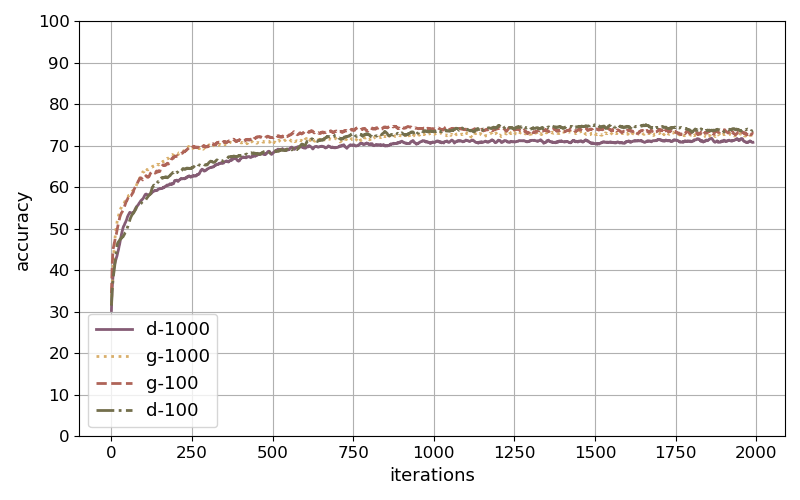
\includegraphics[width=0.45\textwidth]{./5_exp/figs/exp_adv_label_acc_conv-jim}
  \caption{Accuracies of the \texttt{conv-jim} model, with different feature enhancements and frame-based normalization.}
  \label{fig:exp_adv_label_acc_conv-jim}
\end{figure}
\FloatBarrier
\noindent

Noise invariance:
\begin{figure}[!ht]
  \centering
  \subfigure[D]{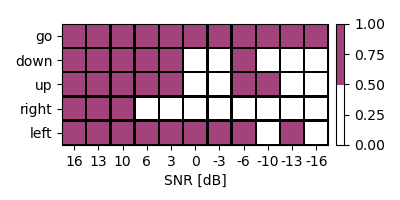
\includegraphics[width=0.4\textwidth]{./5_exp/figs/exp_adv_label_tb_noise_conv-jim_d-100}}
  \subfigure[G]{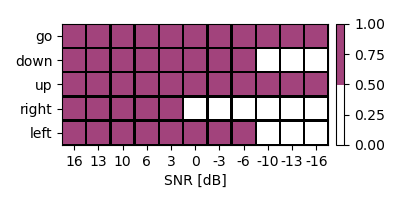
\includegraphics[width=0.4\textwidth]{./5_exp/figs/exp_adv_label_tb_noise_conv-jim_g-100}}
  \caption{Noise invariance of the \texttt{conv-jim} model,  model with adv-label-train of 100 epochs pre-training and using either the Generator (G) or Discriminator (D) weights.}
  \label{fig:exp_adv_label_tb_noise_conv-jim}
\end{figure}
\FloatBarrier
\noindent

Shift invariance:
\begin{figure}[!ht]
  \centering
  \subfigure[D]{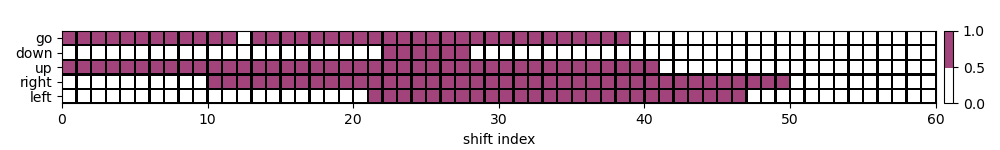
\includegraphics[width=0.45\textwidth]{./5_exp/figs/exp_adv_label_tb_shift_conv-jim_d-100}}
  \subfigure[G]{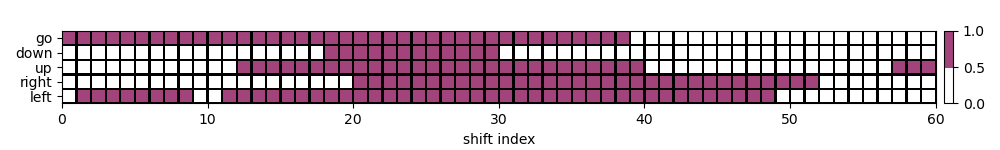
\includegraphics[width=0.45\textwidth]{./5_exp/figs/exp_adv_label_tb_shift_conv-jim_g-100}}
  \caption{Shift invariance of the \texttt{conv-jim} model with adv-label-train of 100 epochs pre-training and using either the Generator (G) or Discriminator (D) weights.}
  \label{fig:exp_adv_label_tb_shift_conv-jim}
\end{figure}
\FloatBarrier
\noindent


% --
% adv dual train

\subsection{Impact of Adversarial Dual Train}
The adv-dual-train experiments were similar to the adv-label-train, but without choosing subsets of labels and simply using the same convolutional layer structure for the Generator and Discriminator model like the CNN network.
The experiments are presented in \rtab{exp_adv_dual_l12}.
\begin{table}[ht!]
\small
\begin{center}
\caption{Experiment with adversarial dual pre-training, using either Generator or Discriminator weights.}
\begin{tabular}{ M{2cm}  M{2cm}  M{2.5cm}  M{2.5cm} }
\toprule
\multicolumn{2}{c}{\textbf{Adversarial}} & \multicolumn{2}{c}{\textbf{Accuracy [\%]}}\\
Epochs & Model & Test set & My dataset\\
\midrule
100 & G & $73.53 \pm 1.75$ & $79.20 \pm 7.33$ \\
100 & D & $69.03 \pm 6.53$ & $72.80 \pm 15.88$ \\
1000 & G & $73.53 \pm 1.53$ & $84.00 \pm 4.38$ \\
1000 & D & $72.57 \pm 1.05$ & $83.20 \pm 2.99$ \\
\bottomrule
\label{tab:exp_adv_dual_l12}
\end{tabular}
\end{center}
\vspace{-4mm}
\end{table}
\FloatBarrier
\noindent
The dual experiments achieved worse accuracies for the transfer of Discriminator weights, when trained for too long, compared to the initializing of the target model with random weights.
The Generator weights however, could increase the average accuracy by at least \SI{1}{\percent}.
The dual training is not further evaluated regarding shift and noise invariance, because the adv-label-train performed better.

% % old
% \subsection{old renew this}
% To evaluate the value of adversarial pre-training, the architecture is trained first with random init and compared to a training with adversarial pre-training. 
% The training losses of those two training methods are shown in \rfig{exp_adv_fc3_train_loss} as well as their obtained accuracies in \rfig{exp_adv_fc3_val_acc}.

% \begin{figure}[!ht]
%   \centering
%     \subfigure[adv init]{\includegraphics[width=0.45\textwidth]{./5_exp/figs/exp_adv_fc3_train_loss_label}}
%     \subfigure[random init]{\includegraphics[width=0.45\textwidth]{./5_exp/figs/exp_adv_fc3_train_loss_random}}
%   \caption{Comparing the train loss of L5-n500-norm1, c1d0dd0e0-norm1-it1000-bs32-lr0.0001-mo0.5 once with random init and once with adv init with dec-itl1000.}
%   \label{fig:exp_adv_fc3_train_loss}
% \end{figure}
% \FloatBarrier
% \noindent

% \begin{figure}[!ht]
%   \centering
%     \subfigure[adv init]{\includegraphics[width=0.45\textwidth]{./5_exp/figs/exp_adv_fc3_val_acc_label}}
%     \subfigure[random init]{\includegraphics[width=0.45\textwidth]{./5_exp/figs/exp_adv_fc3_val_acc_random}}
%   \caption{Comparing the validation accuracy of L5-n500, c1d0dd0e0-norm1-it1000-bs32-lr0.0001-mo0.5 once with random init and once with adv init with dec-itl1000.}
%   \label{fig:exp_adv_fc3_val_acc}
% \end{figure}
% \FloatBarrier
% \noindent

% The loss and accuracy plots show how well the training was going forward for this showcase example. Both training work well and seem to converge, the one of the adversarial init parameters has a considerably faster convergence time here than the one without.
% The scores on the test sets are shown in \rtab{exp_adv_fc3_score}, where both are achieving high scores on the test set, while the adversarial init one got a few percent more, but less on the my set.
% This does not necessarily proof if one method is better or worse, therefore a more challenging task must be picked.
% But at least it shows that adversarial pre training works at least as good as random initialization.
% \begin{table}[ht!]
\begin{center}
\caption{Score comparison on arch: conv-encoder-fc3 with dataset: L5-n500 and training params: c1d0dd0e0-norm1-it1000-bs32-lr0.0001-mo0.5 and different adv params.}
\begin{tabular}{ M{2cm}  M{1.5cm}  M{1.5cm} }
\toprule
\textbf{adv params} & \textbf{acc test} & \textbf{acc my} \\
\midrule
none & 88.33 & 93.33 \\
dec-itl-1000 & 91.67 & 90.00 \\
\bottomrule
\label{tab:exp_adv_fc3_score}
\end{tabular}
\end{center}
\vspace{-4mm}
\end{table}
\FloatBarrier
\noindent

